%%%%%%%%%%%%%%%%%%%%%%%%%%%%%%%%%%%%%%%%%
% University/School Laboratory Report
% LaTeX Template
% Version 3.1 (25/3/14)
%
% This template has been downloaded from:
% http://www.LaTeXTemplates.com
%
% Original author:
% Linux and Unix Users Group at Virginia Tech Wiki 
% (https://vtluug.org/wiki/Example_LaTeX_chem_lab_report)
%
% License:
% CC BY-NC-SA 3.0 (http://creativecommons.org/licenses/by-nc-sa/3.0/)
%
%%%%%%%%%%%%%%%%%%%%%%%%%%%%%%%%%%%%%%%%%

%----------------------------------------------------------------------------------------
%	PACKAGES AND DOCUMENT CONFIGURATIONS
%----------------------------------------------------------------------------------------

\documentclass{article}

\usepackage[version=3]{mhchem} % Package for chemical equation typesetting
\usepackage{siunitx} % Provides the \SI{}{} and \si{} command for typesetting SI units
\usepackage{graphicx} % Required for the inclusion of images
\usepackage{natbib} % Required to change bibliography style to APA
\usepackage{amsmath} % Required for some math elements 
\usepackage{float}
\usepackage{subcaption}
\usepackage{grffile}
\usepackage{longtable}
\usepackage{times}
\usepackage{textcomp}
\usepackage{dcolumn}
\usepackage{placeins}
\usepackage{tabularx}


\setlength\parindent{0pt} % Removes all indentation from paragraphs

\renewcommand{\labelenumi}{\alph{enumi}.} % Make numbering in the enumerate environment by letter rather than number (e.g. section 6)

%\usepackage{times} % Uncomment to use the Times New Roman font

%----------------------------------------------------------------------------------------
%	DOCUMENT INFORMATION
%----------------------------------------------------------------------------------------

\title{Progress Report 2 \\ ENSF 619-4} % Title

\author{Willis \textsc{Cheung}
\\ Justin \textsc{Woods}
\\ Julian \textsc{Mulia}}
 % Author name


\date{\today} % Date for the report

\begin{document}

\maketitle % Insert the title, author and date

\begin{center}
\begin{tabular}{l r}
Instructor: Zahra Shakeri  % Instructor/supervisor
\end{tabular}
\end{center}

% If you wish to include an abstract, uncomment the lines below
% \begin{abstract}
% Abstract text
% \end{abstract}

%----------------------------------------------------------------------------------------
%	SECTION 1
%----------------------------------------------------------------------------------------

\section{Objectives}

\begin{description}
  \item[$\bullet$ ] Data Labeling
  \item[$\bullet$ ] Visualizations and comparison with last trial
  \item[$\bullet$ ]	Unsupervised Learning
  \item[$\bullet$ ] Supervised Learning
\end{description}


%----------------------------------------------------------------------------------------
%	SECTION 2
%----------------------------------------------------------------------------------------

\section{Update}

\paragraph{}
Since the last progress report, we were able to perform the following:

\begin{description}
  \item[$\bullet$ ] Re-run our pre-processing script using the new keywords derived from various subreddits.  
  \item[$\bullet$ ] Compare the distribution of data labels to our previous trial.
  \item[$\bullet$ ] Perform supervised and unsupervised learning.
\end{description}

\section{Data Distribution}

\paragraph{}
After re-running our pre-processing script, we were able to filter out 91,811 tweets.  We believed that applying spam filters with commonly seen trigrams used in job postings and apartment listings (ex: "click the link" and "apartments for rent") could improve the results of our NLP modeling.  This time, we labeled 2045 data points using the same methodology as before:  

\begin{description}
  \item[$\bullet$ ] Indicative of psychological stress. (P)
  \item[$\bullet$ ] Indicative of sleep disorder. (Z)
  \item[$\bullet$ ] Both sleep and stress disorder.  (B)
  \item[$\bullet$ ] Neither sleep nor stress disorder. (N)
  \item[$\bullet$ ] Unclear. (U)
\end{description}

During our previous labeling, we had seen the distribution of data points to be the following:

\begin{table}[ht]
\caption{Label Counts with Original Keyword Filtering}
\centering
\begin{tabular}{rlrr}
  \hline
  Label & Freq & Perc \\ 
  \hline
  N & 1557 & 77.81 \\ 
   P & 209 & 10.44 \\ 
   U & 147 & 7.35 \\ 
   Z &  55 & 2.75 \\ 
   B &  33 & 1.65 \\ 
   \hline
\end{tabular}
\end{table}

Now, with our improved keyword filters, we were able to improve the distribution of relevant points, particularly for tweets containing indicators of stress. 

\begin{table}[ht]
\caption{Label Counts with Refined Keyword Filtering}
\centering
\begin{tabular}{rlrr}
  \hline
  Label & Freq & Perc \\ 
  \hline
 N & 1489 & 72.81 \\ 
   P & 390 & 19.07 \\ 
   Z &  95 & 4.65 \\ 
   B &  45 & 2.20 \\ 
   U &  26 & 1.27 \\ 
   \hline
\end{tabular}
\end{table}


%----------------------------------------------------------------------------------------
%	SECTION 4
%----------------------------------------------------------------------------------------

\section{Supervised Learning}
\paragraph{}
With our new labeled data set, we were able to perform the following supervised learning techniques:

\begin{description}
  \item[$\bullet$ ] Naive Bayes
  \item[$\bullet$ ] Logistic Regression
\end{description}

\subsection{Naive Bayes}
\paragraph{}
For our Naive Bayes model, we used the variation known as the binary Naive Bayes which considers only the presence/absence of features, rather than the frequency.  This is more effective for sentiment classification (particularly in shorter documents) as word occurrence is more important than word frequency.  For our modeling, we considered a 80:20 training/test split.  

\paragraph{}
We reduced the number of features by ignoring words appearing in less than five tweets.  The resulting confusion matrices can be shown below:

\begin{figure}[H]
\begin{center}
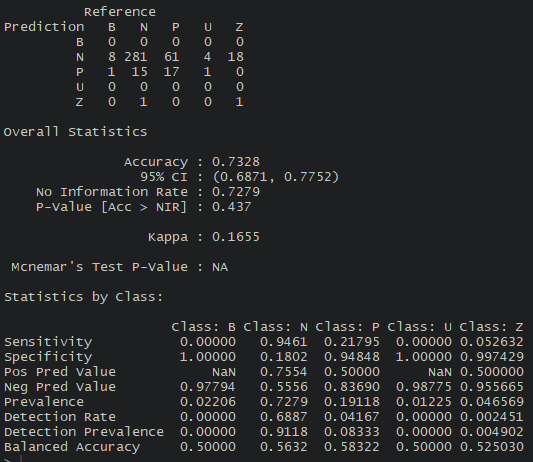
\includegraphics[width=0.65\textwidth]{Images/BNB_Results.png}
\caption{Binary Naive Bayes Summary Results and Confusion Matrix}
\label{fig:BNB Results}
\end{center}
\end{figure}     

\paragraph{}
From the results shown above in Figure \ref{fig:BNB Results}, we can see that the model is just slightly better than if one were to just predict a class of "Neither", which would result in being accurate 72.79\% of the time.  We believe this is due to the relative lack of tweets labeled as "sleep" or "stress" compared to "neither".  Perhaps with more labeled points and improved spam filtering, this result could be improved.


\subsection{Logistic Regression}
\paragraph{}
For our logistic regression, we took the following features as potential independent variables:  

\begin{description}
  \item[$\bullet$ ] Total Sentiment Score (normalized using AFINN lexicon scores)
  \item[$\bullet$ ] account\textunderscore life\textunderscore days (normalized)
  \item[$\bullet$ ] latitude (normalized)
  \item[$\bullet$ ] longitude (normalized)
  \item[$\bullet$ ] province
  \item[$\bullet$ ] tweet\textunderscore day (day of month)
  \item[$\bullet$ ] tweet\textunderscore hour (0 = midnight)
  \item[$\bullet$ ] tweet\textunderscore weekday (0 = monday)
  \item[$\bullet$ ] user\textunderscore followers\textunderscore count (normalized)
  \item[$\bullet$ ] user\textunderscore friends\textunderscore count (normalized)
  \item[$\bullet$ ] user\textunderscore listed\textunderscore count (normalized)
  \item[$\bullet$ ] user\textunderscore statuses\textunderscore count (normalized)
  \item[$\bullet$ ] user\textunderscore verified (normalized)
\end{description}

\paragraph{}
From the fit of the linear model to our labeled data, we can see if there are any significant correlations to the sleep or stress labels.  From Table \ref{Sleep logistic regression results}, we notice that the following:

\begin{description}
  \item[$\bullet$ ] Authors from Manitoba had a higher odds of writing a tweet being indicative of a sleep disorder (p $<$ 0.05).  
  \item[$\bullet$ ] Tweets posted between 1am-4am (p $<$ 0.01) and 5am-7am (p $<$ 0.05) had a higher odds of being indicative of a sleep disorder.
  \item[$\bullet$ ] Users with a higher friends count had a lower odds of publishing tweets being indicative of sleep disorder (p $<$ 0.05)
\end{description}

\paragraph{}
 If more tweets were able to be labeled, one might find additional significant findings from this particular model (for example, further variations for tweet hours, province, or other independent variables).  

\paragraph{}
A similar model can be built with tweets that were labeled as showing signs of psychological stress. From Table \ref{Stress logistic regression results}, we can extract some more interesting findings:

\begin{description}
   \item[$\bullet$ ] Having a higher sentiment score resulted in a lower odds of the tweet being indicative of stress (p $<$ 0.01). 
   \item[$\bullet$ ] Tweets published from Manitoba, New Brunswick, Nova Scotia, Ontario, and Quebec all had a higher odds of indicating Stress (p $<$ 0.05).  
   \item[$\bullet$ ] Tweets published between, 12pm-1pm had a lower odds of being indicative of stress (p $<$ 0.05).
   \item[$\bullet$ ] Tweets published on Wednesdays (p $<$ 0.01), Thursdays (p $<$ 0.05), and Sundays (p $<$ 0.05) all had higher odds of indicating stress.
   \end{description}

\paragraph{}
Finally, the models can be applied to our test data set to evaluate performance.  We started by conducting a single fold prediction for a 60:40 train/test split.  

\begin{figure}[H]
\begin{subfigure}[b]{0.5\linewidth}
	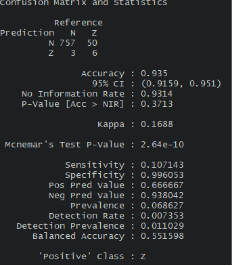
\includegraphics[width=\linewidth]
	{Images/Linear_model_sleep_cm.png}
	\caption{Logistic Regression Model Sleep Confusion Matrix}
\end{subfigure}
\begin{subfigure}[b]{0.5\linewidth}
	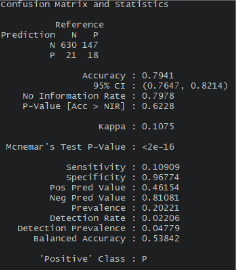
\includegraphics[width=\linewidth]
	{images/Linear_model_stress_cm.png}
	\caption{Logistic Regression Model Stress Confusion Matrix}
\end{subfigure}
\caption{Logistic Regression Results}
\label{fig:LR Results}
\end{figure}

\paragraph{}
The models both perform quite poorly in predicting for sleep and stress, due to the heavy bias in the labeled data.  As a result, the models are really only good for predicting whether the tweet is labeled as "neither".  Again, better performance might be achieved through refined keyword filtering and additional data labeling.  As an exercise, we performed a 10 fold cross validation to see if there would be any variation in accuracy or false positive and false negative rates.  In each of the cases, we did not see that much variation in the accuracy, or false positive and negative rates.      

\begin{figure}[H]
\begin{subfigure}[b]{\linewidth}
	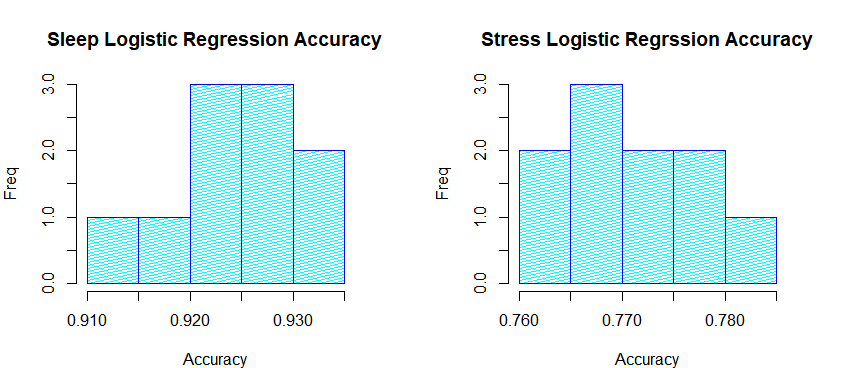
\includegraphics[width=\linewidth]
	{Images/Sleep and Stress LR Accuracies.png}
	\caption{Sleep/Stress Cross Validated Accuracy}
\end{subfigure}
\begin{subfigure}[b]{\linewidth}
	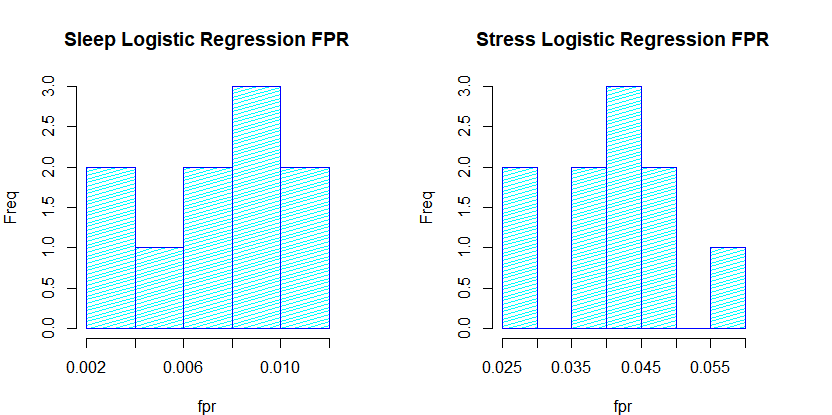
\includegraphics[width=\linewidth]
	{images/Sleep Stress FPR.png}
	\caption{Sleep and Stress Logistic Regression Models FPR}
\end{subfigure}
\begin{subfigure}[b]{\linewidth}
	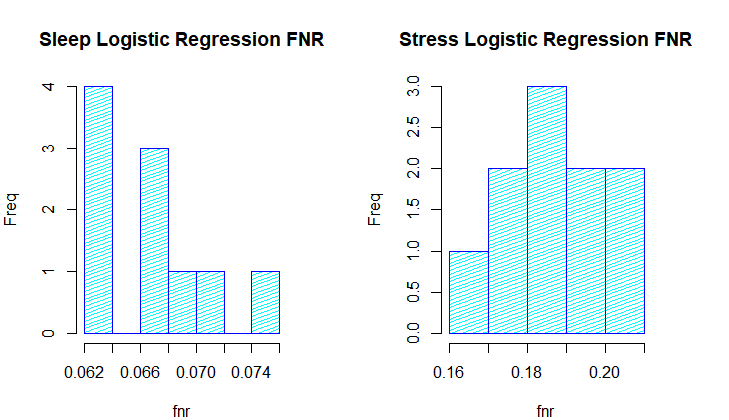
\includegraphics[width=\linewidth]
	{images/Sleep Stress FNR.png}
	\caption{Sleep and Stress Logistic Regression Models FNR}
\end{subfigure}
\caption{Logistic Regression Cross Validation Results}
\label{fig:LR Cross Validation Results}
\end{figure}

\paragraph{}

\subsection{Unsupervised Learning}
\paragraph{}

We employed the BDA and LDA unsupervised learning techniques to extract three topics from the full set of unlabeled tweets.  

\paragraph{}
For the LDA method, we used a subset of 25000 of the  tweets to extract topics due to memory constraints.  For example, from Table \ref{LDA table 6 topics}, we can interpret the topics as follows:

\begin{description}
   \item[$\bullet$ ] Topic 1: Mental Health
   \item[$\bullet$ ] Topic 2: Stress related to work
   \item[$\bullet$ ] Topic 3: Stress/Sleep related to weather, early morning
   \item[$\bullet$ ] Topic 4: General positive sentiment
   \item[$\bullet$ ] Topic 5: Tired/sick sentiment
   \item[$\bullet$ ] Topic 6: Angry sentiment (very stressed)
\end{description}


% latex table generated in R 3.5.2 by xtable 1.8-3 package
% Wed Mar 27 19:28:38 2019
\begin{table}[htb]
\caption{LDA table 3 topics}
\label{LDA table 3 topics}
\centering
\begin{tabular}{rlll}
  \hline
 & Topic 1 & Topic 2 & Topic 3 \\ 
  \hline
1 & cold & life & shit \\ 
  2 & school & hate & fuck \\ 
  3 & job & heart & fucking \\ 
  4 & day & people & time \\ 
  5 & today & years & hours \\ 
   \hline
\end{tabular}
\end{table}

\begin{table}[htb]
\caption{LDA table 4 topics}
\label{LDA table 4 topics}
\centering
\begin{tabular}{rllll}
  \hline
 & Topic 1 & Topic 2 & Topic 3 & Topic 4 \\ 
  \hline
1 & life & school & shit & cold \\ 
  2 & time & heart & fuck & day \\ 
  3 & job & coffee & fucking & today \\ 
  4 & years & rest & hate & hours \\ 
  5 & mental & new & people & late \\ 
   \hline
\end{tabular}
\end{table}

% latex table generated in R 3.5.2 by xtable 1.8-3 package
% Thu Mar 28 16:00:32 2019
\begin{table}[htb]
\caption{LDA table 5 topics}
\label{LDA table 5 topics}
\centering
\begin{tabular}{rlllll}
  \hline
 & Topic 1 & Topic 2 & Topic 3 & Topic 4 & Topic 5 \\ 
  \hline
1 & life & heart & cold & shit & school \\ 
  2 & time & coffee & day & fuck & rest \\ 
  3 & job & mental & today & fucking & new \\ 
  4 & years & love & hours & hate & high \\ 
  5 & ago & health & late & people & year \\ 
   \hline
\end{tabular}
\end{table}

% latex table generated in R 3.5.2 by xtable 1.8-3 package
% Thu Mar 28 18:16:53 2019
\begin{table}[htb]
\caption{LDA table 6 topics}
\label{LDA table 6 topics}
\centering
\begin{tabular}{rllllll}
  \hline
 & Topic 1 & Topic 2 & Topic 3 & Topic 4 & Topic 5 & Topic 6 \\ 
  \hline
1 & job & life & shit & time & cold & school \\ 
  2 & mental & heart & fuck & hours & day & rest \\ 
  3 & health & years & fucking & late & today & new \\ 
  4 & ever & love & hate & bed & coffee & high \\ 
  5 & someone & emojifacewithtearsofjoy & people & sick & good & year \\ 
   \hline
\end{tabular}
\end{table}


% latex table generated in R 3.5.2 by xtable 1.8-3 package
% Thu Mar 28 18:59:08 2019
\begin{table}[htb]
\caption{LDA table 7 topics}
\label{LDA table 7 topics}
\centering
\begin{tabular}{rlllllll}
  \hline
 & Topic 1 & Topic 2 & Topic 3 & Topic 4 & Topic 5 & Topic 6 & Topic 7 \\ 
  \hline
1 & job & late & cold & life & time & shit & school \\ 
  2 & mental & years & day & heart & hours & fuck & new \\ 
  3 & health & ago & today & love & bed & fucking & high \\ 
  4 & ever & game & coffee & never & sick & hate & year \\ 
  5 & care & pressure & good & rest & emojifacewithtearsofjoy & people & kids \\ 
   \hline
\end{tabular}
\end{table}

\FloatBarrier
\paragraph{}
For the BTM method, we used a subset of 6511 of the tweets to extract topics due to memory constraints.  The three to five topic models are shown below.  Again we can try to interpret the topics by grouped tokens.  For example, for Table \ref{BTM table 5 topics}:

\begin{description}
   \item[$\bullet$ ] token: Complaining about weather/school/life
   \item[$\bullet$ ] token1: Complaining about weather, cold, snow
   \item[$\bullet$ ] token2: Difficult to interpret
   \item[$\bullet$ ] token3: Weather forecast
   \item[$\bullet$ ] token4: Public health announcement (likely related to BellLetsTalk Campaign)
\end{description}


% latex table generated in R 3.5.2 by xtable 1.8-3 package
% Thu Mar 28 20:51:34 2019
\begin{table}[ht]
\caption{BTM table 3 topics}
\label{BTM table 3 topics}
\centering
\begin{tabular}{rlll}
  \hline
 & token & token1 & token2 \\ 
  \hline
1 & life & mental & emoji\_red\_heart \\ 
  2 & cold & health & school \\ 
  3 & im & emoji\_pizza & alarm \\ 
  4 & school & stigma & avenue \\ 
  5 & shit & emoji\_woman & institution \\ 
   \hline
\end{tabular}
\end{table}

% latex table generated in R 3.5.2 by xtable 1.8-3 package
% Thu Mar 28 20:49:40 2019
\begin{table}[ht]
\caption{BTM table 4 topics}
\label{BTM table 4 topics}
\centering
\begin{tabular}{rllll}
  \hline
 & token & token1 & token2 & token3 \\ 
  \hline
1 & life & school & mental & cold \\ 
  2 & im & emoji\_red\_heart & health & wind \\ 
  3 & cold & avenue & emoji\_pizza & emoji\_heavy\_minus\_sign \\ 
  4 & school & dispatched & stigma & weather \\ 
  5 & shit & institution & fighting & emoji\_snowflake \\ 
   \hline
\end{tabular}
\end{table}

% latex table generated in R 3.5.2 by xtable 1.8-3 package
% Thu Mar 28 20:48:20 2019
\begin{table}[ht]
\caption{BTM table 5 topics}
\label{BTM table 5 topics}
\centering
\begin{tabular}{rlllll}
  \hline
 & token & token1 & token2 & token3 & token4 \\ 
  \hline
1 & life & cold & emoji\_red\_heart & emoji\_pizza & mental \\ 
  2 & im & coffee & school & wind & health \\ 
  3 & school & emoji\_snowflake & avenue & pressure & stigma \\ 
  4 & cold & emoji\_heavy\_minus\_sign & alarm & rain & fighting \\ 
  5 & shit & snow & institution & forecast & alcoholawareness \\ 
   \hline
\end{tabular}
\end{table}



%----------------------------------------------------------------------------------------
%	SECTION 5
%----------------------------------------------------------------------------------------
\clearpage

\section{Appendix A}

\begin{longtable}{@{\extracolsep{10pt}}lc} 
  \caption{Sleep logistic regression results} 
  \label{Sleep logistic regression results} 
\\[-1.8ex]\hline 
\hline \\[-1.8ex] 
 & \multicolumn{1}{c}{\textit{Dependent variable:}} \\ 
\cline{2-2} 
\\[-1.8ex]\hline 
\hline \\[-1.8ex] 
 & \multicolumn{1}{c}{\textit{Dependent variable:}} \\ 
\cline{2-2} 
\\[-1.8ex] & sleep\_label \\ 
\hline \\[-1.8ex] 
 total\_score & $-$0.171$^{*}$ \\ 
  & (0.093) \\ 
  & \\ 
 account\_life\_days & $-$0.126 \\ 
  & (0.099) \\ 
  & \\ 
 `provinceBritish Columbia` & $-$0.360 \\ 
  & (0.717) \\ 
  & \\ 
 provinceManitoba & 2.369$^{**}$ \\ 
  & (1.146) \\ 
  & \\ 
 `provinceNew Brunswick` & 5.181$^{*}$ \\ 
  & (3.121) \\ 
  & \\ 
 `provinceNewfoundland and Labrador` & 4.057 \\ 
  & (3.633) \\ 
  & \\ 
 `provinceNorthwest Territories` & $-$17.438 \\ 
  & (6,522.639) \\ 
  & \\ 
 `provinceNova Scotia` & 3.802 \\ 
  & (3.241) \\ 
  & \\ 
 provinceOntario & 3.488 \\ 
  & (2.268) \\ 
  & \\ 
 `provincePrince Edward Island` & $-$11.300 \\ 
  & (2,209.739) \\ 
  & \\ 
 provinceQuebec & 4.309$^{*}$ \\ 
  & (2.566) \\ 
  & \\ 
 provinceSaskatchewan & 1.284$^{*}$ \\ 
  & (0.724) \\ 
  & \\ 
 provinceYukon & $-$17.334 \\ 
  & (6,522.639) \\ 
  & \\ 
 latitude & 0.336 \\ 
  & (0.320) \\ 
  & \\ 
 longitude & $-$1.412 \\ 
  & (1.180) \\ 
  & \\ 
 tweet\_day2 & $-$0.207 \\ 
  & (2,192.898) \\ 
  & \\ 
 tweet\_day3 & $-$32.027 \\ 
  & (3,055.275) \\ 
  & \\ 
 tweet\_day4 & 0.792 \\ 
  & (0.954) \\ 
  & \\ 
 tweet\_day5 & 14.985 \\ 
  & (2,023.118) \\ 
  & \\ 
 tweet\_day6 & $-$15.776 \\ 
  & (2,346.932) \\ 
  & \\ 
 tweet\_day7 & $-$33.393 \\ 
  & (3,055.275) \\ 
  & \\ 
 tweet\_day8 & $-$0.152 \\ 
  & (0.635) \\ 
  & \\ 
 tweet\_day9 & $-$0.241 \\ 
  & (2,192.899) \\ 
  & \\ 
 tweet\_day10 & $-$32.452 \\ 
  & (3,055.275) \\ 
  & \\ 
 tweet\_day11 & $-$15.768 \\ 
  & (1,640.505) \\ 
  & \\ 
 tweet\_day12 & 15.890 \\ 
  & (2,023.118) \\ 
  & \\ 
 tweet\_day13 & $-$14.989 \\ 
  & (2,346.932) \\ 
  & \\ 
 tweet\_day14 & $-$33.384 \\ 
  & (3,055.275) \\ 
  & \\ 
 tweet\_day15 & $-$1.447$^{*}$ \\ 
  & (0.871) \\ 
  & \\ 
 tweet\_day16 & $-$0.143 \\ 
  & (2,192.899) \\ 
  & \\ 
 tweet\_day17 & $-$32.460 \\ 
  & (3,055.275) \\ 
  & \\ 
 tweet\_day18 & $-$1.098 \\ 
  & (1.156) \\ 
  & \\ 
 tweet\_day19 & 13.956 \\ 
  & (2,023.118) \\ 
  & \\ 
 tweet\_day20 & $-$16.195 \\ 
  & (2,346.932) \\ 
  & \\ 
 tweet\_day21 & $-$33.754 \\ 
  & (3,055.275) \\ 
  & \\ 
 tweet\_day22 & $-$0.341 \\ 
  & (0.892) \\ 
  & \\ 
 tweet\_day23 & $-$15.349 \\ 
  & (2,346.932) \\ 
  & \\ 
 tweet\_day24 & $-$31.988 \\ 
  & (3,055.275) \\ 
  & \\ 
 tweet\_day25 & 0.158 \\ 
  & (0.649) \\ 
  & \\ 
 tweet\_day26 & 0.142 \\ 
  & (2,192.899) \\ 
  & \\ 
 tweet\_day27 & $-$31.913 \\ 
  & (3,055.275) \\ 
  & \\ 
 tweet\_day28 & $-$0.178 \\ 
  & (0.915) \\ 
  & \\ 
 tweet\_day29 & 15.390 \\ 
  & (2,023.118) \\ 
  & \\ 
 tweet\_day30 & $-$16.138 \\ 
  & (2,346.931) \\ 
  & \\ 
 tweet\_day31 & $-$32.362 \\ 
  & (3,055.275) \\ 
  & \\ 
 tweet\_hour1 & 1.574$^{**}$ \\ 
  & (0.619) \\ 
  & \\ 
 tweet\_hour2 & 1.480$^{**}$ \\ 
  & (0.723) \\ 
  & \\ 
 tweet\_hour3 & 1.490$^{**}$ \\ 
  & (0.693) \\ 
  & \\ 
 tweet\_hour4 & 0.652 \\ 
  & (0.806) \\ 
  & \\ 
 tweet\_hour5 & 1.569$^{**}$ \\ 
  & (0.659) \\ 
  & \\ 
 tweet\_hour6 & 1.270$^{**}$ \\ 
  & (0.636) \\ 
  & \\ 
 tweet\_hour7 & 0.998 \\ 
  & (0.650) \\ 
  & \\ 
 tweet\_hour8 & 1.098$^{*}$ \\ 
  & (0.640) \\ 
  & \\ 
 tweet\_hour9 & $-$0.077 \\ 
  & (0.720) \\ 
  & \\ 
 tweet\_hour10 & 0.179 \\ 
  & (0.651) \\ 
  & \\ 
 tweet\_hour11 & 0.474 \\ 
  & (0.634) \\ 
  & \\ 
 tweet\_hour12 & $-$0.318 \\ 
  & (0.716) \\ 
  & \\ 
 tweet\_hour13 & 0.039 \\ 
  & (0.718) \\ 
  & \\ 
 tweet\_hour14 & $-$0.453 \\ 
  & (0.772) \\ 
  & \\ 
 tweet\_hour15 & $-$0.260 \\ 
  & (0.717) \\ 
  & \\ 
 tweet\_hour16 & $-$0.476 \\ 
  & (0.774) \\ 
  & \\ 
 tweet\_hour17 & $-$0.240 \\ 
  & (0.716) \\ 
  & \\ 
 tweet\_hour18 & $-$1.772 \\ 
  & (1.121) \\ 
  & \\ 
 tweet\_hour19 & $-$0.106 \\ 
  & (0.675) \\ 
  & \\ 
 tweet\_hour20 & 0.208 \\ 
  & (0.633) \\ 
  & \\ 
 tweet\_hour21 & 0.878 \\ 
  & (0.567) \\ 
  & \\ 
 tweet\_hour22 & 0.385 \\ 
  & (0.618) \\ 
  & \\ 
 tweet\_hour23 & 0.497 \\ 
  & (0.654) \\ 
  & \\ 
 tweet\_weekday1 & $-$32.297 \\ 
  & (3,055.275) \\ 
  & \\ 
 tweet\_weekday2 & $-$32.633 \\ 
  & (2,127.417) \\ 
  & \\ 
 tweet\_weekday3 & $-$0.445 \\ 
  & (0.577) \\ 
  & \\ 
 tweet\_weekday4 & $-$33.237 \\ 
  & (3,055.275) \\ 
  & \\ 
 tweet\_weekday5 & $-$48.405 \\ 
  & (2,289.476) \\ 
  & \\ 
 tweet\_weekday6 & $-$17.550 \\ 
  & (1,956.175) \\ 
  & \\ 
 user\_followers\_count & $-$0.014 \\ 
  & (0.291) \\ 
  & \\ 
 user\_friends\_count & $-$0.813$^{**}$ \\ 
  & (0.389) \\ 
  & \\ 
 user\_listed\_count & $-$0.003 \\ 
  & (0.202) \\ 
  & \\ 
 user\_statuses\_count & $-$0.111 \\ 
  & (0.155) \\ 
  & \\ 
 user\_verified & $-$0.867 \\ 
  & (1.120) \\ 
  & \\ 
 Constant & 27.403 \\ 
  & (3,055.276) \\ 
  & \\ 
\hline \\[-1.8ex] 
Observations & 2,045 \\ 
Log Likelihood & $-$437.432 \\ 
Akaike Inf. Crit. & 1,034.864 \\ 
\hline 
\hline \\[-1.8ex] 
\textit{Note:}  & \multicolumn{1}{r}{$^{*}$p$<$0.1; $^{**}$p$<$0.05; $^{***}$p$<$0.01} \\ 
\end{longtable} 


% Table created by stargazer v.5.2.2 by Marek Hlavac, Harvard University. E-mail: hlavac at fas.harvard.edu
% Date and time: Mon, Mar 25, 2019 - 9:49:42 PM
\pagebreak

\begin{longtable}{@{\extracolsep{10pt}}lc} 
  \caption{Stress logistic regression results} 
  \label{Stress logistic regression results} 
\\[-1.8ex]\hline 
\hline \\[-1.8ex] 
 & \multicolumn{1}{c}{\textit{Dependent variable:}} \\ 
\cline{2-2} 
\\[-1.8ex] & stress\_label \\ 
\hline \\[-1.8ex] 
 total\_score & $-$0.653$^{***}$ \\ 
  & (0.066) \\ 
  & \\ 
 account\_life\_days & $-$0.093 \\ 
  & (0.060) \\ 
  & \\ 
 `provinceBritish Columbia` & $-$0.756$^{*}$ \\ 
  & (0.436) \\ 
  & \\ 
 provinceManitoba & 1.892$^{**}$ \\ 
  & (0.748) \\ 
  & \\ 
 `provinceNew Brunswick` & 4.943$^{**}$ \\ 
  & (2.035) \\ 
  & \\ 
 `provinceNewfoundland and Labrador` & 4.287$^{*}$ \\ 
  & (2.349) \\ 
  & \\ 
 `provinceNorthwest Territories` & $-$12.593 \\ 
  & (535.412) \\ 
  & \\ 
 `provinceNova Scotia` & 4.893$^{**}$ \\ 
  & (2.102) \\ 
  & \\ 
 provinceOntario & 3.473$^{**}$ \\ 
  & (1.498) \\ 
  & \\ 
 `provincePrince Edward Island` & 4.422$^{*}$ \\ 
  & (2.332) \\ 
  & \\ 
 provinceQuebec & 3.719$^{**}$ \\ 
  & (1.687) \\ 
  & \\ 
 provinceSaskatchewan & 0.591 \\ 
  & (0.479) \\ 
  & \\ 
 provinceYukon & $-$14.352 \\ 
  & (535.412) \\ 
  & \\ 
 latitude & 0.202 \\ 
  & (0.206) \\ 
  & \\ 
 longitude & $-$1.600$^{**}$ \\ 
  & (0.752) \\ 
  & \\ 
 tweet\_day2 & $-$0.239 \\ 
  & (1.288) \\ 
  & \\ 
 tweet\_day3 & 0.796 \\ 
  & (1.591) \\ 
  & \\ 
 tweet\_day4 & $-$0.062 \\ 
  & (0.739) \\ 
  & \\ 
 tweet\_day5 & $-$0.575 \\ 
  & (1.297) \\ 
  & \\ 
 tweet\_day6 & 0.096 \\ 
  & (1.475) \\ 
  & \\ 
 tweet\_day7 & 2.080 \\ 
  & (1.743) \\ 
  & \\ 
 tweet\_day8 & $-$0.182 \\ 
  & (0.453) \\ 
  & \\ 
 tweet\_day9 & $-$0.601 \\ 
  & (1.364) \\ 
  & \\ 
 tweet\_day10 & 1.155 \\ 
  & (1.668) \\ 
  & \\ 
 tweet\_day11 & 0.073 \\ 
  & (0.755) \\ 
  & \\ 
 tweet\_day12 & $-$0.381 \\ 
  & (1.295) \\ 
  & \\ 
 tweet\_day13 & $-$0.236 \\ 
  & (1.476) \\ 
  & \\ 
 tweet\_day14 & 2.234 \\ 
  & (1.740) \\ 
  & \\ 
 tweet\_day15 & $-$0.958$^{*}$ \\ 
  & (0.539) \\ 
  & \\ 
 tweet\_day16 & $-$0.821 \\ 
  & (1.353) \\ 
  & \\ 
 tweet\_day17 & 1.390 \\ 
  & (1.656) \\ 
  & \\ 
 tweet\_day18 & 0.785$^{*}$ \\ 
  & (0.460) \\ 
  & \\ 
 tweet\_day19 & $-$0.236 \\ 
  & (1.285) \\ 
  & \\ 
 tweet\_day20 & 0.194 \\ 
  & (1.452) \\ 
  & \\ 
 tweet\_day21 & 2.322 \\ 
  & (1.741) \\ 
  & \\ 
 tweet\_day22 & $-$0.657 \\ 
  & (0.609) \\ 
  & \\ 
 tweet\_day23 & 0.303 \\ 
  & (1.453) \\ 
  & \\ 
 tweet\_day24 & 1.774 \\ 
  & (1.747) \\ 
  & \\ 
 tweet\_day25 & $-$0.600 \\ 
  & (0.519) \\ 
  & \\ 
 tweet\_day26 & $-$1.244 \\ 
  & (1.384) \\ 
  & \\ 
 tweet\_day27 & 1.251 \\ 
  & (1.662) \\ 
  & \\ 
 tweet\_day28 & $-$0.267 \\ 
  & (0.567) \\ 
  & \\ 
 tweet\_day29 & 0.081 \\ 
  & (1.258) \\ 
  & \\ 
 tweet\_day30 & $-$0.626 \\ 
  & (1.357) \\ 
  & \\ 
 tweet\_day31 & 1.084 \\ 
  & (1.655) \\ 
  & \\ 
 tweet\_hour1 & 0.087 \\ 
  & (0.420) \\ 
  & \\ 
 tweet\_hour2 & $-$0.743 \\ 
  & (0.555) \\ 
  & \\ 
 tweet\_hour3 & $-$0.277 \\ 
  & (0.516) \\ 
  & \\ 
 tweet\_hour4 & $-$0.153 \\ 
  & (0.550) \\ 
  & \\ 
 tweet\_hour5 & $-$1.173$^{*}$ \\ 
  & (0.610) \\ 
  & \\ 
 tweet\_hour6 & $-$0.298 \\ 
  & (0.432) \\ 
  & \\ 
 tweet\_hour7 & $-$0.050 \\ 
  & (0.415) \\ 
  & \\ 
 tweet\_hour8 & $-$0.515 \\ 
  & (0.436) \\ 
  & \\ 
 tweet\_hour9 & $-$0.610 \\ 
  & (0.399) \\ 
  & \\ 
 tweet\_hour10 & $-$0.151 \\ 
  & (0.363) \\ 
  & \\ 
 tweet\_hour11 & $-$0.661$^{*}$ \\ 
  & (0.396) \\ 
  & \\ 
 tweet\_hour12 & $-$0.792$^{**}$ \\ 
  & (0.399) \\ 
  & \\ 
 tweet\_hour13 & $-$0.776$^{*}$ \\ 
  & (0.398) \\ 
  & \\ 
 tweet\_hour14 & $-$0.704$^{*}$ \\ 
  & (0.404) \\ 
  & \\ 
 tweet\_hour15 & 0.001 \\ 
  & (0.358) \\ 
  & \\ 
 tweet\_hour16 & $-$0.053 \\ 
  & (0.370) \\ 
  & \\ 
 tweet\_hour17 & $-$0.524 \\ 
  & (0.375) \\ 
  & \\ 
 tweet\_hour18 & $-$0.648$^{*}$ \\ 
  & (0.368) \\ 
  & \\ 
 tweet\_hour19 & $-$0.633$^{*}$ \\ 
  & (0.363) \\ 
  & \\ 
 tweet\_hour20 & $-$0.212 \\ 
  & (0.350) \\ 
  & \\ 
 tweet\_hour21 & $-$0.531 \\ 
  & (0.352) \\ 
  & \\ 
 tweet\_hour22 & $-$0.511 \\ 
  & (0.364) \\ 
  & \\ 
 tweet\_hour23 & $-$0.429 \\ 
  & (0.380) \\ 
  & \\ 
 tweet\_weekday1 & 2.469 \\ 
  & (1.677) \\ 
  & \\ 
 tweet\_weekday2 & 3.008$^{***}$ \\ 
  & (1.099) \\ 
  & \\ 
 tweet\_weekday3 & 1.213$^{**}$ \\ 
  & (0.521) \\ 
  & \\ 
 tweet\_weekday4 & 1.830 \\ 
  & (1.743) \\ 
  & \\ 
 tweet\_weekday5 & 2.086$^{*}$ \\ 
  & (1.194) \\ 
  & \\ 
 tweet\_weekday6 & 2.026$^{**}$ \\ 
  & (0.961) \\ 
  & \\ 
 user\_followers\_count & 0.052 \\ 
  & (0.053) \\ 
  & \\ 
 user\_friends\_count & $-$0.047 \\ 
  & (0.090) \\ 
  & \\ 
 user\_listed\_count & $-$0.039 \\ 
  & (0.085) \\ 
  & \\ 
 user\_statuses\_count & $-$0.084 \\ 
  & (0.077) \\ 
  & \\ 
 user\_verified & $-$0.732 \\ 
  & (0.608) \\ 
  & \\ 
 Constant & $-$5.433$^{***}$ \\ 
  & (1.995) \\ 
  & \\ 
\hline \\[-1.8ex] 
Observations & 2,045 \\ 
Log Likelihood & $-$954.590 \\ 
Akaike Inf. Crit. & 2,069.180 \\ 
\hline 
\hline \\[-1.8ex] 
\textit{Note:}  & \multicolumn{1}{r}{$^{*}$p$<$0.1; $^{**}$p$<$0.05; $^{***}$p$<$0.01} \\ 
\end{longtable}     


%----------------------------------------------------------------------------------------
%	BIBLIOGRAPHY
%----------------------------------------------------------------------------------------


%----------------------------------------------------------------------------------------


\end{document}
